%-------------------------------------------------------------------------------
% cookbook_sequencers
%-------------------------------------------------------------------------------
%
% \file        cookbook_sequencers.tex
% \library     Documents
% \author      Chris Ahlstrom
% \date        2016-03-12
% \update      2016-03-13
% \version     $Revision$
% \license     $XPC_GPL_LICENSE$
%
%     Provides the discusson of using sequencers with Yoshimi.
%
%-------------------------------------------------------------------------------

\section{Sequencers}
\label{sec:sequencers}

   This section discusses the basic usage of some sequencers
   with \textsl{Yoshimi}.
   Some sequencers support ALSA MIDI, some support JACK MIDI, and some
   support both.  This section provides some use cases and pointers that cover
   a range of sequencers.
   Note that this section depends on having one's Banks/Roots directories set
   up properly.  It is important to make sure that there is a default
   "presets" directory present.

   So far, we demonstrate only \textsl{Sequencer64}.
   Others to try in the near future:
      \textsl{Rosegarden},
      \textsl{Qtractor},
      \textsl{Ardour},
      \textsl{MuSE},
      \textsl{LMMS}.

\subsection{Sequencers / Sequencer64}
\label{subsec:sequencers_seq64}

   \textsl{Sequencer64} is our fork/reboot of the \textsl{Seq24}
   project \cite{sequencer64}.
   \index{Sequencer64}
   It currently fixes some bugs in \textsl{Seq24},
   \index{Seq24}
   adds a few useful features,
   a little more color, and refactors the code.
   Much of the advice in this section will apply to
   \textsl{Seq24}, with some minor differences, such as the locations and names
   of the configuration files.  However, \textsl{Seq24} doesn't have a
   buss-override option.

   Note that the two \textsl{Sequencer64} configuration files are:

   \begin{verbatim}
      ~/.config/sequencer64/sequencer64.rc
      ~/.config/sequencer64/sequencer64.usr
   \end{verbatim}

   \index{sequencer64.rc}
   \index{sequencer64.usr}

   The simplest thing to do for this cookbook is
   
   \begin{itemize}
      \item Make sure these files do not exist; save the old versions somewhere
      and then delete the two files.
      \item Then start \textsl{Sequencer64}.
      \item Then immediately exit it.
   \end{itemize}
      
   New versions of those files will appear, and we can start with a clean
   slate.  We will edit those files, as that is a bit more foolproof than using
   command-line options.  The "rc" is the most important file, but there are
   configuration items in the "usr" ("user") file that can make
   \textsl{Sequencer} prettier, and a couple options that can affect playback.
   We'll point out the necessary values when needed.

\subsubsection{Sequencers / Sequencer64 / ALSA}
\label{subsubsec:sequencers_seq64_alsa}

   \index{ALSA}
   Skip this section if all that matters for one's setup is JACK support.
   Otherwise, first make sure that JACK is not running.
   Next, remove the "rc" and "usr" files from the configuration directory, as
   noted in the previous section.
   Then open up a console window (terminal) and run \textsl{Yoshimi} in ALSA
   audio and ALSA MIDI modes:

   \begin{verbatim}
      $ yoshimi -a -A
   \end{verbatim}

   Now, run \textsl{Sequencer64}, and check the new
   versions of those files, as noted in the previous section.
   On our computer, with Timidity installed, we see the following ALSA entries
   in the \texttt{sequencer64.rc} file:

   \begin{verbatim}
		# Output buss name: [0] 14:0 Midi Through Port-0
		0 0  # buss number, clock status
		# Output buss name: [1] 128:0 TiMidity port 0
		1 0  # buss number, clock status
		# Output buss name: [2] 128:1 TiMidity port 1
		2 0  # buss number, clock status
		# Output buss name: [3] 128:2 TiMidity port 2
		3 0  # buss number, clock status
		# Output buss name: [4] 128:3 TiMidity port 3
		4 0  # buss number, clock status
		# Output buss name: [5] 129:0 input
		5 0  # buss number, clock status
   \end{verbatim}

   The last entry in that list is "129:0 input", which corresponds to
   \textsl{Yoshimi}.  Note that the \textsl{Sequencer64} application will
   find the actual name of the device (e.g. "129:0 Yoshimi Port 0").
   
   While we're in the "rc" file, let's make sure of the following settings:

   \begin{verbatim}
      1     # show sequence numbers (1 = true / 0 = false)

		[manual-alsa-ports]
		0     # flag for manual ALSA ports
   \end{verbatim}

   The first setting enables showing the sequence number in empty slots in the
   main window.  (This setting really belongs in the "user" file!)
   The second setting disables manual setup of the ALSA MIDI ports.
   \textsl{Sequencer64} will determine the ports that exist on the system.

   In the "user" file, we want to set the buss number to 5, to match our
   current ALSA setup.  It may differ on your system.  If it is 0, you don't
   have to do the next step.  Nor is it needed for running with JACK (discussed
   later).

   Open the "user" file and make sure the following setting matches the
   location of \textsl{Yoshimi}'s MIDI input port on your system (it is 5 on
   ours):

   \begin{verbatim}
      5       # midi_buss_override
   \end{verbatim}

   Now open a MIDI file, verify that the correct buss value is shown, and that
   the file plays and is audible.  If this is the case, one is done.  If not,
   please read the \textsl{Sequencer64} user's manual
   (\cite{sequencer64doc}).

   Note that, generally, the "midi\_buss\_override" value should be set to
   "-1".  We use it here as a convenience for our demonstration.
   Also, one can load a preset/patch-set file from the command line, as shown
   here:

   \begin{verbatim}
      $ yoshimi -a -A --load=/home/user/.../yoshimi-cookbook/yoshimi/examples/Out_There.xmz
      Yoshimi is starting
      ConfigFile /home/user/.config/yoshimi/yoshimi.config not found,
            will use default settings
      Missing bank file
      Scanning for banks
      Missing history file
      March little endian = 1
      Format = Signed Little Endian 32 Bit 2 Channel
      Using alsa_audio for audio and alsa_midi for midi
      pLoaded Out_There parameters
      Yoshimi 1.3.9 rc3
      Clientname: yoshimi
      Config: Audio: alsa -> 'default'
      Midi: alsa -> 'default'
      Oscilsize: 512
      Samplerate: 48000
      Period size: 256

      Yay! We're up and running :-)
   \end{verbatim}

   Now go to \sectionref{subsubsec:sequencers_seq64_out_there}.
   Load up a sample song and patch-set, and play it.

\subsubsection{Sequencers / Sequencer64 / JACK}
\label{subsubsec:sequencers_seq64_jack}

   \index{JACK}
   Now let's repeat our setup using JACK.  However, note that, while
   \textsl{Sequencer64} supports JACK synchronization and can serve as a JACK
   Master, it's MIDI support is purely ALSA-based.
   Therefore, an ALSA-to-JACK bridge program must be run to expose
   the MIDI ports to JACK.
   
   Before continuing, make sure the \textsl{Sequencer64} "rc" and "usr" files
   reflect the following settings, which are different than those described in
   the ALSA section above.  First, the "rc" file:

   \begin{verbatim}
      1     # show sequence numbers (1 = true / 0 = false); ignored in legacy
		[manual-alsa-ports]
		0     # flag for manual ALSA ports (--manual-alsa-ports)
   \end{verbatim}

   Manual ALSA ports can be turned on, but that results in 16 additional
   \textsl{Sequencer64} MIDI ports being created;
   the MIDI Through port will be enough
   for now, since we're using only one synthesizer, \textsl{Yoshimi},
   for sound generation.
   Next, the "usr" file:

   \begin{verbatim}
      -1      # midi_buss_override (--bus n)
   \end{verbatim}

   (If the buss is set properly, as above, in the
   \texttt{\textasciitilde/.config/sequencer64/sequencer64.usr} file,
   there is no need for the \texttt{--bus} option on the command line.)

   Now run the following series of commands, from a console window:

   \begin{verbatim}
      $ qjackctl &
      $ a2jmidid --export-hw &
      $ sequencer64 &
      $ yoshimi -j -J 
   \end{verbatim}

   In \textsl{qjacktrl}, in the \textbf{Audio} tab, connect "yoshimi" on the
   left with "system" on the right.

\begin{figure}[H]
   \centering 
   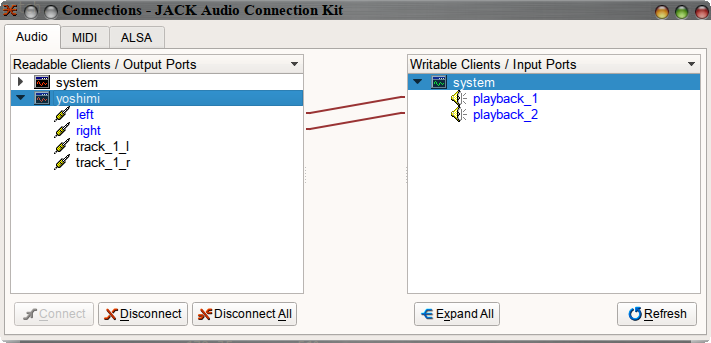
\includegraphics[scale=0.75]{jack/yoshimi-audio.png}
   \caption{Yoshimi Audio Connection, JACK}
   \label{fig:cookbook_yoshimi_audio_connection}
\end{figure}

   In the \textbf{MIDI} tab, connect a2j's "Midi Through [14] (capture)..."
   port on the left to yoshimi-01's "midi in" port on the right.

\begin{figure}[H]
   \centering 
   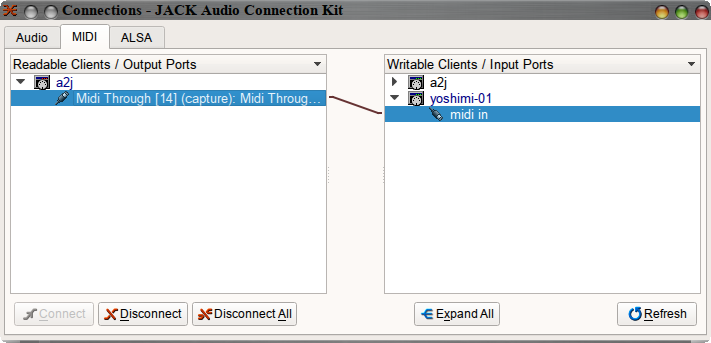
\includegraphics[scale=0.75]{jack/yoshimi-midi.png}
   \caption{Yoshimi MIDI Connection, JACK}
   \label{fig:cookbook_yoshimi_midi_connection}
\end{figure}

   Now go to \sectionref{subsubsec:sequencers_seq64_out_there}.
   Load up a sample song and patch-set, and play it.

\subsubsection{Sequencers / Sequencer64 / "Out There"}
\label{subsubsec:sequencers_seq64_out_there}

   In this section, we set up and run a demo file and patch-set file
   provided with \textsl{Yoshimi}.  Let's start from scratch.

\paragraph{Initial Installation}
\label{paragraph:yoshimi_init_install}

   \begin{enumerate}
      \item Install \textsl{Yoshimi} from a package manager or from source code.
      \item Install \textsl{ZynAddSubFx} from a package manager or from source
         code.  This action gets us more instrument banks.
      \item Clone the yoshimi-cookbook \cite{yoshimicookbook}
         project from GitHub.
      \item Clone the sequencer64 \cite{sequencer64} project from GitHub.
   \end{enumerate}

\paragraph{Start from Scratch}
\label{paragraph:yoshimi_start_from_scratch}

   Remove any existing \textsl{Yoshimi} configuration.

   \begin{verbatim}
      $ cd ~/.config
      $ mv yoshimi/ yoshimi-orig
   \end{verbatim}

   Start Yoshimi:

   \begin{verbatim}
      $ yoshimi --version
      Yoshimi is starting
      ConfigFile /home/user/.config/yoshimi/yoshimi.config not found,
            will use default settings
      Missing bank file
      Scanning for banks
      Missing history file
      Yoshimi 1.3.9
   \end{verbatim}

   This "first start" results in the creation of 
   \texttt{\textasciitilde/.config/yoshimi} and
   an empty \texttt{\textasciitilde/.config/yoshimi/presets} directory.

\paragraph{Load Example XMZ File}
\label{paragraph:yoshimi_load_xmz_file}

   The next step in this demonstration is to load a parameters (patch-set)
   file.  We pick the parameters file provided by the \textsl{Yoshimi}
   source-code package for the "Out There" project.  We show the command-line
   \textsl{Yoshimi} in ALSA mode for simplicity:

   \begin{verbatim}
      $ yoshimi -a -A --load=/home/user/.../yoshimi-cookbook/yoshimi/examples/Out_There.xmz
   \end{verbatim}

   Remember that \textsl{Yoshimi} cannot find the parameters file if
   \texttt{/home/user} part is replaced with \texttt{\textasciitilde}.
	This action results in additional files created in
   \texttt{\textasciitilde/.config/yoshimi}:
      \texttt{yoshimi.history},
      \texttt{yoshimi.banks},
      \texttt{yoshimi.windows}.

   The history file contains a reference to the full path of the
   \texttt{Out\_There.xmz} file.

   The \texttt{yoshimi.banks} file is a gzip-compressed XML file that
   references the default bank-root (bank-root 0):
   \texttt{/usr/share/yoshimi/banks} or
   \texttt{/usr/local/share/yoshimi/banks}.
   It also defines
   prefix number for all of the banks (bank directories) that ship with
   \textsl{Yoshimi}.  It also references the
   \textsl{ZynAddSubFX} bank location (if installed):
   \texttt{/usr/share/zynaddsubfx/bank} (bank-root 1).
   It defines bank numbers for all of
   the banks that ship with \textsl{ZynAddSubFX}.

   The \texttt{yoshimi.windows} file contains the locations of about 20
   windows, such as "master", "panel", "instruments", "SUBnote", "ADDnote",
   and many more.

   The patch-set can also be loaded through the \textsl{Yoshimi}
   user-interface.
   In the \textbf{Yoshimi / Patch Sets / Load External...} menu, load the
   example \texttt{Out\_There.xmz} patch-set file file, and observe that
   the "Angel Piano" instrument appears as \textbf{Part 1}.

\paragraph{Playing Out\_There}
\label{paragraph:yoshimi_playing_out_there}

   Run \textsl{Yoshimi} as above for either ALSA or JACK.
   Then run \textsl{Sequencer64} as above for either ALSA or JACK.

   Sequencer64 converts the SFM 0 file, \texttt{Out\_There.mid},
   to SMF 1 as it reads in the file.
   It also deposits the original SMF 0 track into the 16th slot, highlighted in
   a dark-cyan color.
   Delete this SMF 0 track by right-clicking on it and selecting the
   \textbf{Cut} menu entry.

   Arm (unmute) all of the tracks in the main window view of Sequencer64.
   This is done by simply left-clicking once on each slot.
   They are then shown with a black background.

   Play!  Either click the play button or hit the spacebar.
   This setup can loop endlessly, and the differing lengths of the parts
   make it vary as it plays, forever.  (\textsl{Sequencer64} is a live-looping
   sequencer.)

   When done, don't save either the \textsl{Yoshimi} parameters or the
   converted tune.

   \begin{verbatim}
      yoshimi> exit
      System config has been changed.  Still exit N/y? y
   \end{verbatim}

\subsubsection{Sequencers / Sequencer64 / Basic Composing}
\label{subsubsec:sequencers_seq64_basic_composing}

   Finally, we are ready to add our own music, starting
   with a loop.  In \textsl{Sequencer64}, right click
   on a pattern slot and select \textbf{New}.  On the bottom of the new pattern
   window, select the left-most icon button, which shows a blue box pointing to
   a MIDI port (tooltip: "Sequence dumps data to MIDI bus.").
   Press the Space bar while in the main window or the pattern window
   to start the loop, and add notes.

   \begin{quotation}
      \textbf{Peculiarities of Sequencer64}.
      First, if the pattern is empty the
      progress bar will not move.  Second, to add a note, one must press
      the right button (the pointer changes to a pencil) and, while holding
      it, press the left mouse button.  Or click in the pattern editor, press
      "p" to select the pencil mode, then click/drag to add notes.  Press "x"
      to "eXit" from that mode.  Also remember that notes are drawn only with
      the length selected by the "notes" button near the top of the pattern
      window.  Again, see the Sequencer64 user manual for the gory details.
   \end{quotation}

   MORE TO COME!

%-------------------------------------------------------------------------------
% vim: ts=3 sw=3 et ft=tex
%-------------------------------------------------------------------------------
